\chapter{\IfLanguageName{dutch}{Proof of concept}{Proof of concept}}%
\label{ch:proof-of-concept}

Dit hoofdstuk beschrijft de ontwikkeling van de proof-of-concept (POC) voor het automatisch detecteren van de open of gesloten status van supermarkten op basis van historische POI-data. De POC is volledig geïmplementeerd in Python en bestaat uit de volgende fasen: data en bibliotheken inladen, data analyse, feature engineering, het trainen van de modellen en evaluatie. De implementatie is gedocumenteerd in een Jupyter Notebook.

\section{Databronnen en datastructuur}
\subsection{Geografische afbakening}

Een eerste belangrijke beslissing betreft de geografische scope van de dataset. De interne POI-databank van Accurat bevat records voor meerdere Europese landen. Voor de ontwikkeling van deze POC werd gekozen om vier coherente landen te gebruiken: België, Nederland, Luxemburg en Frankrijk. Deze vormen een regio waarin vergelijkbare supermarktketens actief zijn, wat de vergelijkbaarheid van de geleerde patronen ten goede komt. 

%Voor de ontwikkeling van deze POC werd echter bewust besloten om Duitsland uit te sluiten uit de analyse. De reden hiervoor is van datastructurele aard: bepaalde Duitse supermarktketens, waaronder Aldi Süd, zijn vertegenwoordigd met honderdduizenden records. Omdat de historische statusregistraties en openingsuren van één filiaal over meerdere rijen verdeeld zijn, zou een steekproef op rijniveau de integriteit van de volledige POI-geschiedenis per filiaal schenden. Features zoals \texttt{inactiviteit\_ratio} en \texttt{historisch\_inactief\_count} zijn immers afhankelijk van de \textit{volledige} historische reeks per \texttt{poi\_id}; een abrupte afkapping zou deze features corrupt maken en de modelprestaties systematisch vertekenen. Een steekproef op het niveau van de \texttt{poi\_id} (waarbij alle records van geselecteerde filialen integraal worden meegenomen) biedt weliswaar een methodologisch correctere oplossing, maar voegt complexiteit toe die buiten de scope van deze bachelorproef valt.

%TODO: eventueel nog iets aan toe voegen?
\subsection{Basisinformatie van de data}

De volledige POI-dataset die door de opdrachtgever ter beschikking werd gesteld, bevat in totaal 1.337.281 POI-records voor België, Nederland, Luxemburg en Frankrijk. De dataset bestaat uit kolommen zoals: de naam, het adres, de geografische coördinaten, openingsuren, de operationele status, is\_deletes, metadata over de bron en timestamps van aanmaak en wijziging van de Point of interest.

%TODO: is dit nuttig?
\subsection{Trainingsdata}

%Voor de ontwikkeling van de POC werd een geëxporteerde CSV-dataset gebruikt die de samenvoeging vormt van drie onderliggende tabellen uit de database:

%\begin{itemize}
%    \item \textbf{Poi\_history}: historische registraties van de open- of geslotenstatus van een POI, met daarin de velden \texttt{is\_active}, \texttt{status\_start} en \texttt{status\_end}.
    
 %   \item \textbf{POI basisinfo}: basisattributen per locatie, zoals naam, adres, categorie, id gelinkt aan de brand, .
    
  %  \item \textbf{Openingsuren}: de verwachte openingstijden per dag van de week (\texttt{day\_of\_week}), met daarin de velden \texttt{opening\_start}, \texttt{opening\_stop}, \texttt{pause\_start}, \texttt{pause\_stop} en of de POI gesloten is \texttt{closed}. De pauze start en pauze stop zijn geen verplichte velden, aangezien dat niet elke POI een pauze inlast doorheen de dag.
%\end{itemize}

\section{Data-analyse}

\subsection{Verhouding van actieve en inactieve records}

Een eerste stap in de data-analyse bestond uit het in kaart brengen van de verdeling tussen de twee klassen in de doelvariabele \texttt{is\_active}. De labelstrategie is als volgt gedefinieerd:

\begin{itemize}
    \item \texttt{is\_active = 1} duidt op een open POI: de scraper was actief en registreerde de POI als operationeel.
    \item \texttt{is\_active = 0} duidt op een gesloten POI: de scraper was actief maar registreerde de POI als inactief op dat moment.
\end{itemize}

De dataset bevat circa 26.400 gesloten en 31.000 open vestigingen, wat overeenkomt met respectievelijk 46,1\% en 53,9,\%. Dit maakt de dataset relatief gunstig voor een binair classificatieprobleem, aangezien er geen sprake is van een ernstige klasse-onevenwichtigheid die de modelprestaties zou vertekenen.

\begin{figure}[h]
    \centering
    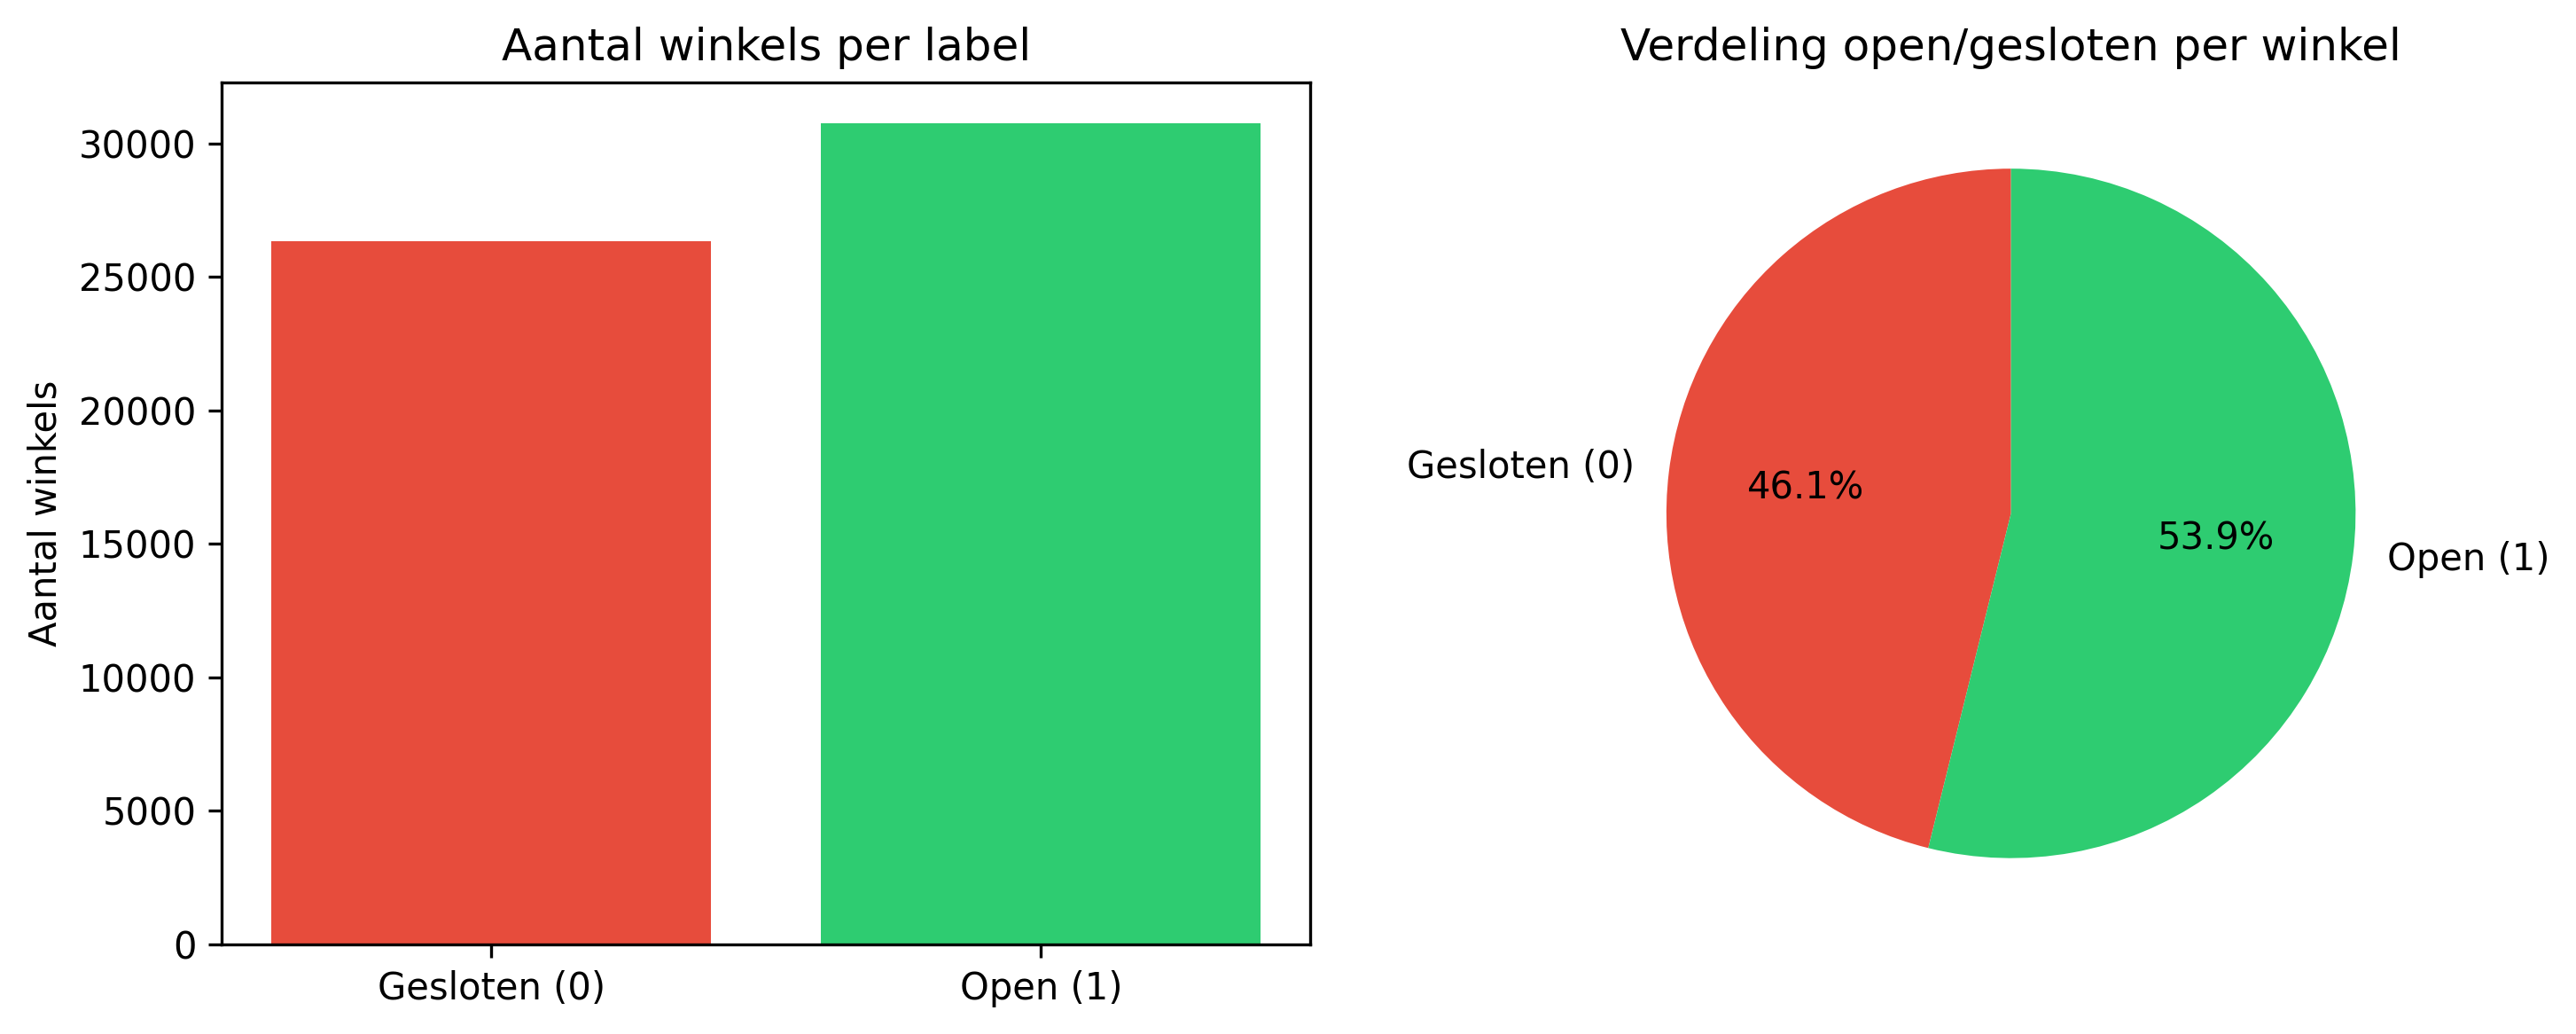
\includegraphics[width=\textwidth]{../proof_of_concept/Grafieken/verdeling_status.png}
    \caption[Verdeling: open vs.\ gesloten]{\label{fig:verdeling open/gesloten}Verdeling van de open en geslotenstatus voor alle merken in de dataset.}
\end{figure}

\subsection{Ontbrekende waarden}
De analyse van ontbrekende waarden onthulde een aantal kolommen die volledig of grotendeels leeg waren in de dataset. Kolommen met 100\% ontbrekende waarden worden automatisch verwijderd uit de dataset alvorens verdere verwerking plaatsvond, 
aangezien deze geen bruikbare informatie kunnen bijdragen aan het model. In de volledige dataset was dit het geval voor \texttt{district\_id}.

Andere kolommen vertoonden een aanzienlijk percentage ontbrekende waarden. Zo ontbrak \texttt{status\_end} in 49,55\% en \texttt{status\_start} in 42,68\% van de records. Dit is te verklaren doordat een ontbrekend eindtijdstip (\texttt{status\_end = Null}) doorgaans aangeeft dat de POI op dat moment nog steeds operationeel is. De openingsuren (\texttt{start.oh} en \texttt{stop.oh}) waren aanwezig in slechts 84,70\% respectievelijk 84,71\% van de records, wat erop wijst dat voor een deel van de POI's geen gestructureerde openingsuren beschikbaar zijn in de databank. Ontbrekende numerieke waarden in de overige feature-kolommen werden aangevuld met de mediaan van de betreffende kolom alvorens het model te trainen.

\subsection{Verdeling top 15 merken}
Om een beter inzicht te krijgen in de verdeling van de operationele status per merk, werden de top 15 meest voorkomende merken gevisualiseerd op basis van hun open en geslotenstatus.

Uit de analyse blijkt dat er een aanzienlijke variatie bestaat in de verhouding tussen open en gesloten vestigingen per merk. Aldi is het meest voorkomende merk in de dataset en vertoont een opvallend hoog aantal gesloten registraties ten opzichte van open, wat kan wijzen op een \textit{decaying}-fase binnen de POI-levenscyclus zoals beschreven door \textcite{Lu2020}. Hetzelfde patroon is zichtbaar bij Intermarché, Spar, Vival en Super U. Aan de andere kant zijn merken zoals E.Leclerc, Carrefour market en Carrefour express bijna uitsluitend vertegenwoordigd met open vestigingen, wat duidt op een stabiele operationele toestand. Hieruit kunnen we concluderen dat we bij de interpretatie van de modelresultaten rekening moeten houden met een mogelijke geospatiale bias: merken die sterk vertegenwoordigd zijn in de dataset zullen een grotere invloed uitoefenen op de geleerde patronen dan merken met weinig records.

\begin{figure}[h]
    \centering
    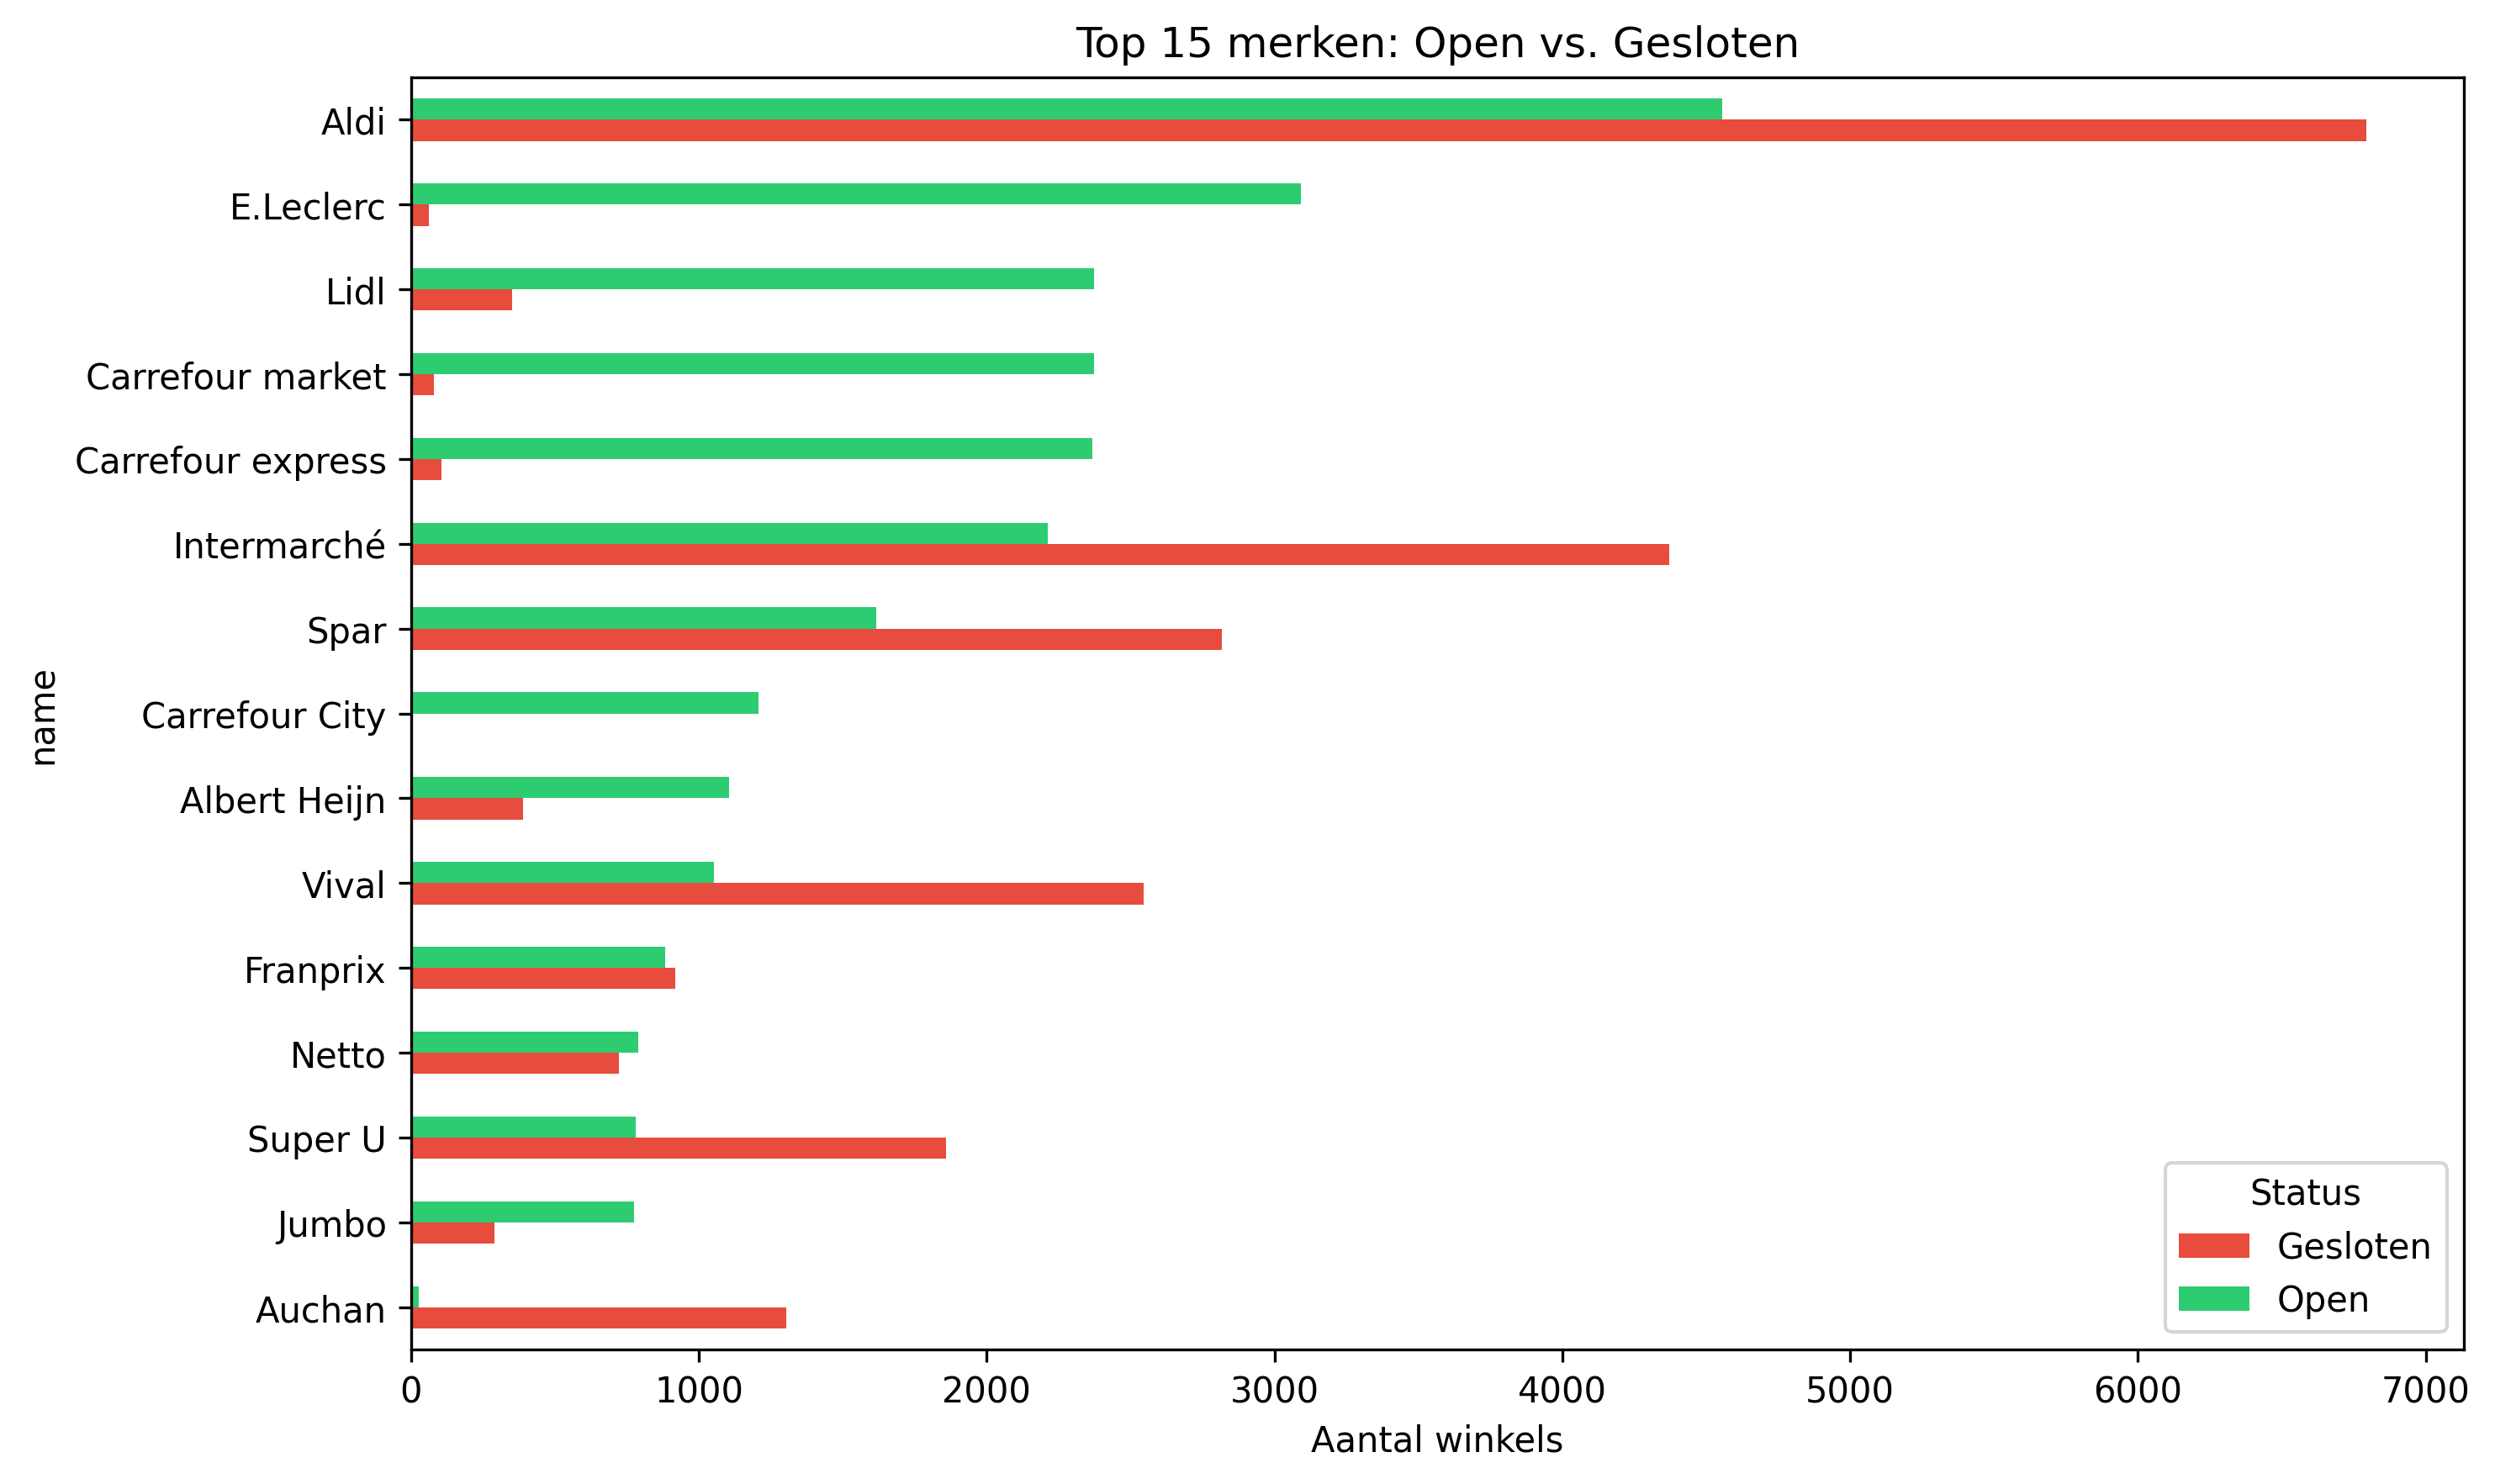
\includegraphics[width=\textwidth]{../proof_of_concept/Grafieken/top_brands.png}
    \caption[Top 15 merken: open vs.\ gesloten]{\label{fig:top15merken}Verdeling van de open en geslotenstatus voor de 15 meest voorkomende merken in de dataset.}
\end{figure}
    
\subsection{Verdeling per land}

Om de geografische spreiding van de dataset in kaart te brengen, werd het aantal POI-records per land gevisualiseerd, samen met de sluitingsratio per land.

Frankrijk is veruit het best vertegenwoordigde land in de dataset met circa 42.000 POI-records, gevolgd door Nederland en België met respectievelijk circa 8.000 en 7.000 records. Luxemburg is met minder dan 500 records slechts beperkt vertegenwoordigd. Deze onevenwichtige geografische verdeling is een potentiële bron van geospatiale bias: het model zal voornamelijk patronen leren op basis van Franse supermarkten, wat de generaliseerbaarheid naar kleinere landen zoals Luxemburg kan beperken.

De sluitingsratio verschilt eveneens per land. Luxemburg kent de hoogste sluitingsratio met circa 53\%, gevolgd door Frankrijk (circa 49\%), België (circa 44\%) en Nederland (circa 38\%). Deze variatie suggereert dat landspecifieke factoren, zoals marktdynamiek en de mate van dataveroudering per regio, een rol spelen in de statusverdeling. Dit sluit aan bij de bevindingen uit de literatuurstudie, waarbij \textcite{Boskovic2026} aantonen dat de socio-economische context van een regio samenhangt met de operationele stabiliteit van supermarktvestigingen.

\begin{figure}[h]
      \centering
      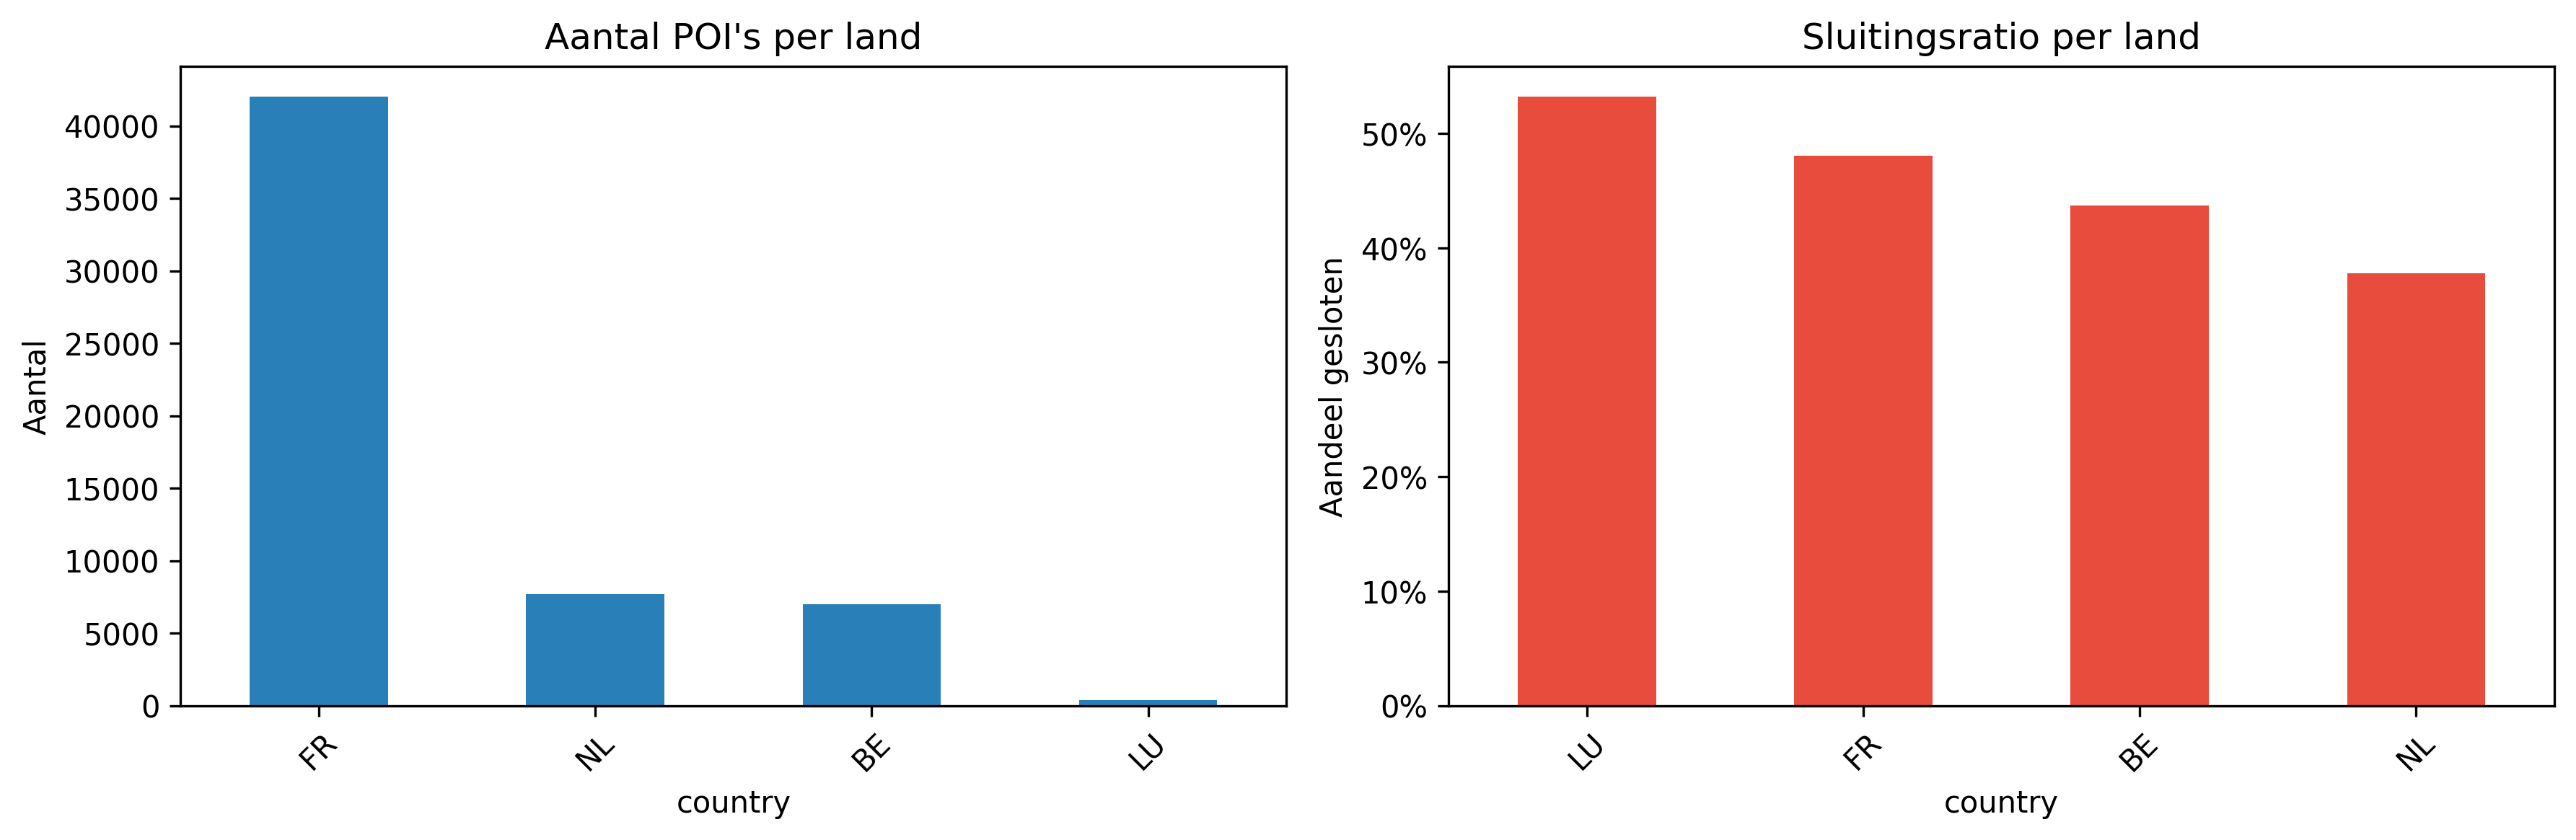
\includegraphics[width=\textwidth]{../proof_of_concept/Grafieken/land_status.png}
      \caption[Verdeling per land]{\label{fig:verdelingland}Aantal POI's per land (links) en sluitingsratio per land (rechts).}
\end{figure}

\section{Feature Engineering}
%TODO
Op basis van de ruwe dataset werden zowel temporele als gedragsmatige kenmerken 
geconstrueerd die relevant zijn voor de statusdetectie. De features werden 
afgeleid uit de beschikbare tijdstempels, openingstijden en historische 
statusregistraties. Tabel~\ref{tab:features} geeft een overzicht van alle 
gebruikte features, samen met hun herkomst en semantische betekenis.

\begin{table}[h]
    \centering
    \small
    \begin{tabular}{lll}
        \toprule
        \textbf{Feature} & \textbf{Type} & \textbf{Beschrijving} \\
        \midrule
        \texttt{maand} & Temporeel & Kalendermaand van de statusregistratie (1–12) \\
        \texttt{day\_of\_week} & Temporeel & Dag van de week (0 = maandag, 6 = zondag) \\
        \texttt{is\_weekend} & Temporeel & Binaire vlag: 1 indien zaterdag of zondag \\
        \texttt{is\_feestdag} & Temporeel & Binaire vlag: 1 indien een feestdag geregistreerd \\
        \texttt{start\_min} & Openingsuren & Openingsuur omgezet naar minuten \\
        \texttt{stop\_min} & Openingsuren & Sluitingsuur omgezet naar minuten \\
        \texttt{verwachte\_openingsduur\_min} & Openingsuren & Verwacht aantal minuten dat de winkel open is \\
        \texttt{closed} & Openingsuren & Binaire vlag uit de openingsuren-tabel \\
        \texttt{ok} & Kwaliteitsvlag & Kwaliteitsvlag van het openingsurenrecord \\
        \texttt{is\_deleted} & POI-status & Binaire vlag: 1 indien POI verwijderd is \\
        \texttt{is\_sensitive} & POI-metadata & Binaire vlag voor gevoelige locaties \\
        \texttt{is\_reserved\_poi} & POI-metadata & Binaire vlag voor gereserveerde POI's \\
        \texttt{cluster} & POI-metadata & Clusteridentificatie van de POI \\
        \texttt{brand\_id\_enc} & POI-metadata & Label-encoded merknummer \\
        \texttt{country\_enc} & POI-metadata & Label-encoded landcode \\
        \texttt{visit} & Gebruikstype & Numerieke classificatie van het bezoektype \\
        \texttt{work} & Gebruikstype & Numerieke classificatie van het werktype \\
        \texttt{historisch\_inactief\_count} & Historisch gedrag & Cumulatief aantal inactieve registraties per POI \\
        \texttt{inactiviteit\_ratio} & Historisch gedrag & Verhouding inactieve registraties t.o.v.\ het totaal \\
        \texttt{poi\_leeftijd\_maanden} & Historisch gedrag & Leeftijd van de POI in maanden sinds eerste record \\
        \bottomrule
    \end{tabular}
    \caption[Overzicht van gebruikte features]{%
        \label{tab:features}Overzicht van de geconstrueerde features, ingedeeld per 
        categorie. De temporele features zijn afgeleid van de \texttt{updated\_at}-kolom; 
        de historische gedragsfeatures zijn berekend via een groepering per \texttt{poi\_id}.}
\end{table}

% TODO: pas de feature-lijst aan indien de definitieve dataset extra features oplevert of
% indien features worden weggelaten na verdere analyse (bv. na een permutation importance analyse).

Drie van de features verdienen bijzondere aandacht vanwege hun semantische relevantie 
voor POI-statusdetectie. Ten eerste is de \texttt{inactiviteit\_ratio} een gedragsmatige 
indicator die de verhouding weergeeft van het aantal inactieve statusregistraties ten 
opzichte van het totale aantal registraties per POI. Een hoge ratio kan duiden op een 
locatie die zich in de \textit{decaying}-fase van de POI-levenscyclus bevindt, zoals 
besproken in de literatuurstudie. Ten tweede geeft \texttt{historisch\_inactief\_count} 
de cumulatieve teller van inactiviteiten per POI weer, berekend op basis van de 
tijdsgeordende statusgeschiedenis. Ten derde weerspiegelt \texttt{poi\_leeftijd\_maanden} 
de periode tussen het eerste geregistreerde record van een POI en het huidige 
observatiemoment, uitgedrukt in maanden. Deze feature is relevant omdat jonge POI's, 
die nog geen stabiel bezoekpatroon hebben opgebouwd, gevoeliger zijn voor het 
cold-start probleem dat in de literatuurstudie werd besproken.

De twee categorische kolommen \texttt{brand\_id} en \texttt{country} werden omgezet 
naar numerieke waarden via Label Encoding alvorens ze als feature aan het model aan 
te bieden. Hoewel Label Encoding een ordinale relatie impliceert die niet noodzakelijk 
aanwezig is tussen merken of landen, werd voor deze aanpak gekozen omwille van de 
schaalbaarheid en de compatibiliteit met de gebruikte modelarchitecturen.

%TODO
\subsection{Train- en testopsplitsing}

De dataset werd opgedeeld in een trainingsset (80\%) en een testset (20\%) via 
gestratificeerde steekproeftrekking (\textit{stratified train-test split}), waarbij de 
doelvariabele \texttt{is\_active} als stratificatiefactor werd gebruikt. Dit garandeert 
dat de klasseverdeling in beide deelsets identiek is aan die van de volledige dataset. 
Na de splitsing resulteerde dit in een trainingsset van 35.507 records en een testset 
van 8.877 records. Een vaste willekeurige zaad (\texttt{RANDOM\_SEED = 42}) werd 
ingesteld om de reproduceerbaarheid van de resultaten te waarborgen.

\subsection{Hyper parametertuning}
%TODO

%TODO
\section{Modellen}

In lijn met de in de literatuurstudie besproken classificatiebenaderingen werden drie 
machine learning modellen geïmplementeerd en met elkaar vergeleken: Logistische Regressie, 
Random Forest en XGBoost. Deze selectie laat toe om een spectrum te evalueren van een 
eenvoudig lineair model tot een geavanceerd boosting-algoritme, wat inzicht verschaft 
in de complexiteit die het statusdetectieprobleem vereist.

\subsection{Model 1: Logistische Regressie}

Logistische Regressie werd opgenomen als basismodel (\textit{baseline}). Het model 
biedt een lineaire beslissingsgrens en maakt geen aannames over niet-lineaire 
verbanden in de data. De absolute waarden van de modelcoëfficiënten werden gebruikt 
om de relatieve bijdrage van elke feature te visualiseren. Logistische Regressie is 
in de literatuur erkend als een interpreteerbaar model dat inzicht verschaft in welke 
features het sterkst bijdragen aan de classificatie, maar dat doorgaans minder 
performant is bij complexe, niet-lineaire datasets.

\subsection{Model 2: Random Forest}

Random Forest is een ensemble-methode die een groot aantal beslissingsbomen 
(\textit{decision trees}) traint op willekeurige deelsets van de data en features, 
en de voorspellingen via meerderheidsstemming combineert. Het model is robuust 
ten opzichte van ruis en overfitting, en produceert automatisch een 
feature-importantiescore op basis van de gemiddelde afname in onzuiverheid 
(Gini-importantie). Het Random Forest model werd getraind met standaardparameters 
en een vaste willekeurige zaad.

\subsection{Model 3: XGBoost}

XGBoost (Extreme Gradient Boosting) is een gradiënt-boostingalgoritme dat iteratief 
zwakke leerders toevoegt om de resterende fouten van de vorige iteratie te corrigeren. 
Het is bijzonder geschikt voor gestructureerde tabeldata en presteert in de praktijk 
vaak beter dan traditionele ensemble-methoden. Gezien de lichte klasse-onevenwichtigheid 
in de testset werd de \texttt{scale\_pos\_weight}-parameter ingesteld op de verhouding 
tussen het aantal negatieve en positieve instanties in de trainingsset. De overige 
hyperparameters zijn samengevat in Tabel~\ref{tab:xgb-params}.

\begin{table}[h]
    \centering
    \small
    \begin{tabular}{ll}
        \toprule
        \textbf{Hyperparameter} & \textbf{Waarde} \\
        \midrule
        \texttt{n\_estimators}     & 300 \\
        \texttt{max\_depth}        & 6 \\
        \texttt{learning\_rate}    & 0,05 \\
        \texttt{subsample}         & 0,8 \\
        \texttt{colsample\_bytree} & 0,8 \\
        \texttt{eval\_metric}      & logloss \\
        \texttt{scale\_pos\_weight} & verhouding negatief/positief \\
        \bottomrule
    \end{tabular}
    \caption[XGBoost hyperparameters]{%
        \label{tab:xgb-params}Overzicht van de gebruikte hyperparameters voor het 
        XGBoost-model. De \texttt{scale\_pos\_weight} werd dynamisch berekend op 
        basis van de klasseverdeling in de trainingsset.}
\end{table}

\section{Evaluatie}

%TODO
\subsection{Evaluatiemetrieken}

De modellen werden geëvalueerd aan de hand van vier standaard classificatiemetrieken: 
accuracy, precision, recall en F1-score. In de context van POI-statusdetectie 
heeft de keuze van de primaire evaluatiemetrie een methodologische consequentie. 
Een hoge \textit{precision} voor de klasse \textit{gesloten} garandeert dat een 
als gesloten gedetecteerde POI effectief gesloten is, wat belangrijk is om 
foutieve updates in de POI-databank te vermijden. Een hoge \textit{recall} voor 
diezelfde klasse garandeert dat werkelijk gesloten POI's niet worden gemist, 
wat cruciaal is wanneer verouderde data directe operationele gevolgen heeft 
voor de eindgebruiker. De F1-score combineert beide metrieken als het harmonisch 
gemiddelde en fungeert als samengestelde indicator voor de algemene modelprestatie.

\subsection{Resultaten}

% TODO: vervang de [TODO]-placeholders in de tabel hieronder door de definitieve 
% resultaten na de volledige run op de productiedataset (België, Nederland, 
% Luxemburg en Frankrijk). Voeg ook een bespreking toe van de verkregen cijfers.

De resultaten van de definitieve evaluatie op de volledige dataset worden weergegeven 
in Tabel~\ref{tab:resultaten}.

\begin{table}[h]
    \centering
    \small
    \begin{tabular}{lcccc}
        \toprule
        \textbf{Model} & \textbf{Accuracy} & \textbf{Precision} & \textbf{Recall} & \textbf{F1-score} \\
        \midrule
        Logistische Regressie & \textit{[TODO]} & \textit{[TODO]} & \textit{[TODO]} & \textit{[TODO]} \\
        Random Forest         & \textit{[TODO]} & \textit{[TODO]} & \textit{[TODO]} & \textit{[TODO]} \\
        XGBoost               & \textit{[TODO]} & \textit{[TODO]} & \textit{[TODO]} & \textit{[TODO]} \\
        \bottomrule
    \end{tabular}
    \caption[Vergelijking van modelresultaten]{%
        \label{tab:resultaten}Vergelijking van de drie modellen op de testset 
        (20\% van de volledige dataset). Alle scores worden gerapporteerd op de 
        gewogen gemiddelden over beide klassen.}
\end{table}

%TODO
\subsection{Feature-importantie}

Een analyse van de feature-importantie laat toe om te begrijpen welke kenmerken 
het sterkst bijdragen aan de classificatiebeslissing. Voor het Random Forest model 
werd de Gini-importantie gebruikt, die aangeeft hoeveel de gemiddelde onzuiverheid 
van de knooppunten afneemt wanneer een bepaalde feature wordt gebruikt voor een 
splitsing. Voor het XGBoost-model werd de ingebouwde feature-importantiescore 
berekend op basis van het gemiddeld aantal keren dat een feature wordt gebruikt 
in de boosting-rondes (\textit{gain}). Voor de Logistische Regressie werd de 
absolute waarde van de modelcoëfficiënt als maatstaf gebruikt.

% TODO: voeg hier een bespreking toe van de top-features na de definitieve run,
% bij voorkeur ondersteund door de gegenereerde staafdiagrammen uit het notebook.

Op basis van de initiële testrun kan worden vastgesteld dat temporele features 
(\texttt{day\_of\_week}, \texttt{maand}, \texttt{is\_weekend}) en 
openingstijdfeatures (\texttt{start\_min}, \texttt{stop\_min}, 
\texttt{verwachte\_openingsduur\_min}) naar verwachting een hoge 
importantiescore zullen behalen. Dit sluit aan bij de bevindingen van 
\textcite{Milias2021}, die aantonen dat operationele kenmerken, waaronder 
bezoekpatronen en specifieke openingstijden, de meest significante variabelen 
zijn voor het classificeren van stedelijke functies. Eveneens wordt verwacht dat 
de gedragsmatige features \texttt{inactiviteit\_ratio} en 
\texttt{historisch\_inactief\_count} een substantiële bijdrage zullen leveren, 
aangezien deze de historische stabiliteit van een POI weerspiegelen en 
daarmee aansluiten bij het concept van de POI-levenscyclus 
zoals gedefinieerd door \textcite{Lu2020}.

%TODO
\subsection{Beperkingen van de huidige POC}

De huidige implementatie kent een aantal methodologische beperkingen die in acht 
dienen te worden genomen bij de interpretatie van de resultaten.

Ten eerste is de testset in de huidige fase beperkt tot twee merken uit één land, 
waardoor de generaliseerbaarheid van de resultaten naar andere ketens en 
geografische contexten niet kan worden gegarandeerd. Wanneer de definitieve dataset 
meerdere landen en merken omvat, is het mogelijk dat de modellen worden geconfronteerd 
met een verhoogde geospatiale variabiliteit, wat de classificatieprestaties kan 
beïnvloeden.

Ten tweede werd in de huidige implementatie geen gebruik gemaakt van 
kruisvalidatie (\textit{k-fold cross-validation}), maar van een enkelvoudige 
train-testsplitsing. Hoewel de gestratificeerde splitsing de klasseverdeling 
bewaart, is een enkelvoudige opsplitsing gevoeliger voor toevallige variaties in 
de samenstelling van de test- en trainingsset. Voor de definitieve evaluatie 
verdient het aanbeveling om k-fold kruisvalidatie toe te passen om een 
betrouwbaardere schatting van de generalisatiefout te verkrijgen.

Ten derde bevat de dataset geen expliciete voetgangers- of transactiegegevens, 
die in de literatuur als krachtige indicatoren voor statuswijzigingen worden 
beschouwd \autocite{Yao2024}. De huidige feature-set is bijgevolg uitsluitend 
gebaseerd op structurele en temporele attributen van de POI, en niet op 
dynamische mobiliteitsdata. Dit is een fundamentele beperking ten opzichte van 
modellen die beschikken over real-time of historische voetverkeersinformatie.

Ten vierde werd geen hyperparameteroptimalisatie uitgevoerd voor het Random Forest 
model, wat betekent dat de gerapporteerde prestaties als een ondergrens kunnen 
worden beschouwd. Voor het XGBoost-model werden de hyperparameters handmatig 
geselecteerd op basis van gangbare standaardwaarden uit de literatuur; een 
systematische zoekprocedure zoals \textit{grid search} of \textit{Bayesian 
    optimization} kan de modelprestaties verder verbeteren.

Ten slotte dient te worden benadrukt dat het probleem van \textit{data-inflatie}, 
zoals besproken door \textcite{Boskovic2026}, ook hier van toepassing kan zijn. 
Wanneer een data-provider zijn registratiemethoden aanpast, kunnen bestaande 
POI-records onterecht als nieuw in de database verschijnen. Dit kan leiden tot 
foutieve labels in de trainingsdata, waarbij een record als \textit{open} 
wordt geclassificeerd terwijl de onderliggende locatie in werkelijkheid al 
geruime tijd inactief was.

%TODO: nakijken
\section{Implementatiedetails}

De volledige POC werd geïmplementeerd in Python 3.12. De volgende bibliotheken werden gebruikt: \texttt{pandas} en \texttt{numpy} voor data-inlading en verwerking, \texttt{scikit-learn} voor de implementatie van Logistische Regressie en Random Forest alsook voor de evaluatiemetrieken en de train-testsplitsing, \texttt{xgboost} voor de XGBoost-implementatie, \texttt{matplotlib} en \texttt{seaborn} voor de visualisaties, \texttt{joblib} voor het persisteren van de getrainde modellen en \texttt{holidays} voor het identificeren van feestdagen per land.

De getrainde modellen worden na afloop van het trainingsproces opgeslagen in een lokale map (\texttt{./models}) via \texttt{joblib.dump()}, zodat ze zonder opnieuw getraind kunnen worden hergebruikt.